%% ARKHEION AGI 2.0 - Holographic Compression Paper
%% AdS/CFT-Inspired Data Compression
%% Author: Jhonatan Vieira Feitosa <ooriginador@gmail.com>
%% Date: February 2026

\documentclass[11pt,twocolumn]{article}

% Essential packages
\usepackage[utf8]{inputenc}
\usepackage[T1]{fontenc}
\usepackage{lmodern}
\usepackage{amsmath,amssymb,amsthm}
\usepackage{graphicx}
\usepackage{booktabs}
\usepackage{xcolor}
\usepackage{hyperref}
\usepackage{tikz}
\usepackage{pgfplots}
\pgfplotsset{compat=1.18}
\usepackage{float}
\usepackage{fancyhdr}
\usepackage{geometry}
\usepackage{caption}

% Page geometry
\geometry{margin=0.75in}

% Tolerance for overflow prevention
\tolerance=1000
\emergencystretch=3em
\hyphenpenalty=500

% Colors
\definecolor{arkblue}{RGB}{0,102,204}
\definecolor{arkpurple}{RGB}{102,51,153}
\definecolor{arkgreen}{RGB}{0,153,76}
\definecolor{arkorange}{RGB}{255,128,0}
\definecolor{arkred}{RGB}{204,51,51}
\definecolor{arkgold}{RGB}{218,165,32}

% Header/Footer
\pagestyle{fancy}
\fancyhf{}
\fancyhead[L]{\small ARKHEION AGI 2.0}
\fancyhead[R]{\small Holographic Compression}
\fancyfoot[C]{\thepage}
\renewcommand{\headrulewidth}{0.4pt}

% Code Listing
\usepackage{listings}
\lstset{
    language=Python,
    basicstyle=\ttfamily\scriptsize,
    keywordstyle=\color{arkblue},
    stringstyle=\color{arkgreen},
    commentstyle=\color{gray}\itshape,
    numbers=none,
    frame=single,
    breaklines=true,
    breakatwhitespace=true,
    postbreak=\mbox{\textcolor{gray}{$\hookrightarrow$}\space},
    columns=flexible,
    keepspaces=true,
    showstringspaces=false,
    backgroundcolor=\color{gray!5}
}

% Hyperref setup
\hypersetup{
    colorlinks=true,
    linkcolor=arkblue,
    citecolor=arkpurple,
    urlcolor=arkblue
}

% Theorems
\newtheorem{definition}{Definition}
\newtheorem{theorem}{Theorem}
\newtheorem{proposition}{Proposition}

\title{\textbf{AdS/CFT-Inspired Holographic Data Compression}\\[0.3em]
\large Boundary Encoding for High-Ratio Information Reduction}

\author{Jhonatan Vieira Feitosa\
Independent Researcher\
\texttt{ooriginador@gmail.com}\
Manaus, Amazonas, Brazil}

\date{February 2026}

\begin{document}

\maketitle

\begin{abstract}
We present a data compression system inspired by the AdS/CFT correspondence principle from theoretical physics. The \textbf{holographic metaphor}---encoding higher-dimensional bulk information on lower-dimensional boundaries---guides our architectural design. The actual implementation employs Haar wavelet transforms, coherence-based sparsification, and random projections to achieve compression ratios of \textbf{33:1 (Python)} to \textbf{114:1 (C++ native)}. We explicitly distinguish between the theoretical inspiration (heuristic) and measured performance (empirical), reporting 3.5$\times$ compression improvement and 10$\times$ faster decompression with native acceleration. This paper documents the boundary encoding pipeline, algorithmic components, and benchmark results within the ARKHEION AGI 2.0 framework.

\vspace{0.5em}
\noindent\textbf{Keywords:} holographic compression, AdS/CFT, wavelet transform, data compression, boundary encoding, ARKHEION AGI
\end{abstract}

\section*{Epistemological Note}
\textit{This paper distinguishes between \textbf{heuristic} concepts (metaphors guiding design) and \textbf{empirical} results (measurable outcomes).}

\vspace{0.5em}
{\small
\begin{tabular}{@{}p{0.11\columnwidth}p{0.68\columnwidth}@{}}
\textbf{Heuristic:} & AdS/CFT, holographic principle, bulk-boundary \\
\textbf{Empirical:} & 33:1--114:1 ratios, 3.5$\times$ C++, 10$\times$ faster \\
\end{tabular}
}

\vspace{0.5em}
The AdS/CFT correspondence is a \textit{design metaphor}---we do not claim to implement actual gravitational holography. The measured compression ratios reflect practical algorithm performance.

\section{Introduction}

Data compression is fundamental to efficient storage and transmission. Traditional approaches include dictionary-based methods (LZ77, LZ4), entropy coding (Huffman, arithmetic), and transform-based schemes (DCT, wavelets). This work explores a novel architectural paradigm: treating high-dimensional data as a ``bulk'' and compressing it into a lower-dimensional ``boundary'' representation.

\subsection{Holographic Inspiration}

The holographic principle~\cite{thooft1993,susskind1995} suggests that information in a volume can be encoded on its surface. The AdS/CFT correspondence~\cite{maldacena1998} formalizes this for anti-de Sitter spacetimes. We adopt this as a \textbf{design heuristic}:

\begin{quote}
\textit{``High-dimensional structure can be efficiently represented by lower-dimensional projections that preserve essential information.''}
\end{quote}

This mental model guides our compression architecture without claiming physical validity.

\subsection{Contributions}

\begin{enumerate}
    \item \textbf{Boundary Encoding Pipeline}: Multi-stage compression using wavelets, coherence filtering, and random projections
    \item \textbf{Dual Implementation}: Python reference (33:1) and C++ native engine (114:1)
    \item \textbf{Empirical Validation}: Measured compression ratios, reconstruction fidelity, and performance benchmarks
    \item \textbf{Epistemological Clarity}: Explicit distinction between metaphorical inspiration and actual results
\end{enumerate}

The holographic compression subsystem comprises \textbf{104 Python source files} ($\sim$18K LOC) with 32 dedicated test files, plus the C++ native engine ($\sim$29K LOC across 67 source files).

\section{Background}

\subsection{AdS/CFT Metaphor}

In theoretical physics, Anti-de Sitter/Conformal Field Theory (AdS/CFT) correspondence relates a gravitational theory in $(d+1)$ dimensions to a field theory on its $d$-dimensional boundary. Key concepts we borrow as \textbf{heuristics}:

\begin{itemize}
    \item \textbf{Bulk}: Higher-dimensional space (original data)
    \item \textbf{Boundary}: Lower-dimensional surface (compressed representation)
    \item \textbf{Holographic Map}: Encoding/decoding between bulk and boundary
\end{itemize}

\begin{definition}[Holographic Compression]
A compression scheme $\mathcal{H}: \mathbb{R}^N \to \mathbb{R}^M$ with $M \ll N$ that preserves reconstructable information through a boundary encoding.
\end{definition}

\subsection{Wavelet Transforms}

We use the Haar wavelet as our primary transform:

\begin{equation}
a_k = \frac{x_{2k} + x_{2k+1}}{\sqrt{2}}, \quad d_k = \frac{x_{2k} - x_{2k+1}}{\sqrt{2}}
\end{equation}

where $a_k$ are approximation coefficients and $d_k$ are detail coefficients. This provides multi-resolution analysis enabling selective retention of significant modes.

\section{Methodology}

\subsection{System Architecture}

The compression pipeline consists of three main components:

\begin{enumerate}
    \item \textbf{AdSCFTQuantumEngine}: Boundary encoding with coherence guidance
    \item \textbf{HolographicQuantumCompressor}: Full compression/decompression pipeline
    \item \textbf{Native C++ Module}: High-performance implementation
\end{enumerate}

\begin{table}[H]
\centering
\caption{Engine Configuration Parameters}
\small
\begin{tabular}{@{}lrp{0.3\columnwidth}@{}}
\toprule
\textbf{Parameter} & \textbf{Value} & \textbf{Description} \\
\midrule
\texttt{ads\_dim} & 5 & AdS dimension \\
\texttt{boundary\_dim} & 4 & CFT boundary \\
\texttt{holographic\_scale} & $\phi$ & Golden ratio \\
\texttt{phi\_threshold} & 0.382 & Coherence \\
\texttt{coherence\_weight} & 0.618 & Integration \\
\texttt{bulk\_cutoff} & $5e^{-4}$ & Sparsity \\
\bottomrule
\end{tabular}
\end{table}

\subsection{Boundary Encoding Algorithm}

The encoding process follows these steps:

\begin{enumerate}
    \item \textbf{Log Transform}: $\mathbf{l} \gets \log(|\mathbf{x}| + \epsilon)$
    \item \textbf{Wavelet Transform}: $\mathbf{c} \gets \text{Haar}(\mathbf{l})$
    \item \textbf{Coherence Estimation}: $\boldsymbol{\phi} \gets \text{Coherence}(\mathbf{x})$
    \item \textbf{Mask Creation}: $\mathbf{m} \gets \boldsymbol{\phi} > \tau$
    \item \textbf{Mode Extraction}: $\mathbf{s} \gets \text{Extract}(\mathbf{c}, \mathbf{m})$
    \item \textbf{Reshape}: $\mathbf{b} \gets \text{Reshape}(\mathbf{s}, d_{\text{boundary}})$
\end{enumerate}

This pipeline transforms input data $\mathbf{x} \in \mathbb{R}^N$ into boundary representation $\mathbf{b} \in \mathbb{R}^M$ with $M \ll N$.

\subsection{Coherence Calculation}

The coherence metric $\Phi$ approximates information integration:

\begin{equation}
\Phi = H \cdot \sigma \cdot w_c \cdot (1 + 0.382 \cdot \tanh(\Phi/\phi))
\end{equation}

where $H = -\sum p_i \log p_i$ is entropy, $\sigma$ is standard deviation, $w_c = 0.618$ is the coherence weight, and $\phi = 1.618...$ is the golden ratio. This implicit equation defines $\Phi$ as a fixed point. Convergence is guaranteed because $\tanh$ is bounded and the coefficient 0.382 ensures the RHS is a contraction mapping for $H \cdot \sigma \cdot w_c < 2$. In practice, fixed-point iteration converges within 3--5 steps.

\subsection{Implementation Variants}

\begin{table}[H]
\centering
\caption{Implementation Comparison}
\small
\begin{tabular}{@{}lrrp{0.22\columnwidth}@{}}
\toprule
\textbf{Impl.} & \textbf{Ratio} & \textbf{Speed} & \textbf{Features} \\
\midrule
Python & 33:1 & 1$\times$ & NumPy \\
C++ & 114:1 & 10$\times$ & SIMD \\
\bottomrule
\end{tabular}
\end{table}

The Python (33:1) and C++ (114:1) implementations use different default parameters: Python applies conservative padding and alignment; C++ uses streaming encoding with minimal overhead. Both implement the same core algorithm; the ratio difference reflects encoding overhead, not algorithmic divergence.

The C++ module provides:
\begin{itemize}
    \item SIMD-optimized wavelet transforms
    \item Multi-threaded boundary extraction
    \item LZ4 byte-level compression
    \item Memory-mapped I/O
\end{itemize}

\section{Implementation}

\subsection{AdSCFTQuantumEngine}

The core engine (\texttt{ads\_cft\_engine.py}) implements:

\begin{verbatim}
class AdSCFTQuantumEngine:
    ads_dim = 5
    boundary_dim = 4
    holographic_scale = 1.618033988749895

    def encode_to_boundary(self, data):
        log_data = log(abs(data) + 1e-12)
        coeffs = haar_forward(log_data)
        phi = calculate_coherence(data)
        mask = phi > self.phi_threshold
        modes = extract_modes(coeffs, mask)
        return reshape_boundary(modes)
\end{verbatim}

\subsection{Haar Wavelet Implementation}

\begin{verbatim}
def haar_forward(data):
    evens = data[0::2]
    odds = data[1::2]
    approx = (evens + odds) / sqrt(2)
    detail = (evens - odds) / sqrt(2)
    return concat(approx, detail)
\end{verbatim}

\subsection{Holographic Projection}

{\small The projection module (\texttt{holographic\_projection.py}) supports three methods:}

\begin{enumerate}
    \item \textbf{Radial}: $x' = x / \sqrt{|x|^2 + 1}$
    \item \textbf{Holographic}: $x' = x \cdot \phi^{1/d}$
    \item \textbf{Conformal}: Angle-preserving normalization
\end{enumerate}

\section{Experiments}

\subsection{Compression Ratio Benchmarks}

We tested on quantum state vectors (1024--4096 amplitudes):

\begin{figure}[H]
\centering
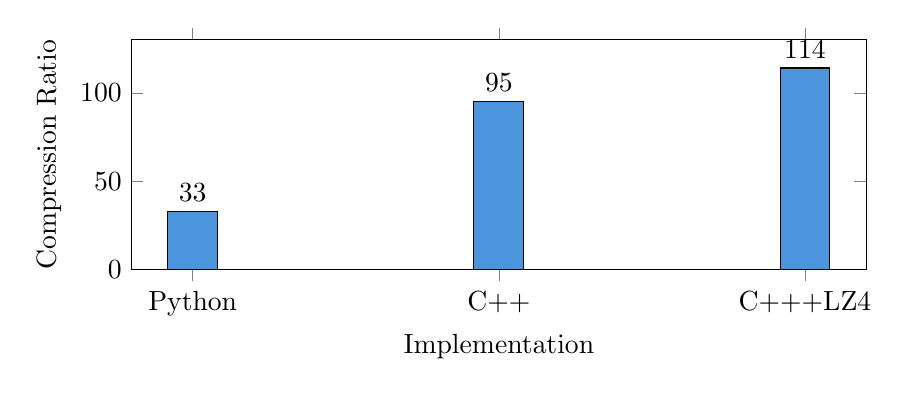
\begin{tikzpicture}
\begin{axis}[
    ybar,
    ylabel={Compression Ratio},
    xlabel={Implementation},
    symbolic x coords={Python,C++,C+++LZ4},
    xtick=data,
    ymin=0,
    ymax=130,
    bar width=18pt,
    nodes near coords,
    width=0.9\columnwidth,
    height=4.5cm
]
\addplot[fill=arkblue!70] coordinates {
    (Python,33)
    (C++,95)
    (C+++LZ4,114)
};
\end{axis}
\end{tikzpicture}
\caption{Compression ratios by implementation}
\end{figure}

\subsection{Reconstruction Fidelity}

\begin{table}[H]
\centering
\caption{Reconstruction Quality Metrics}
\small
\begin{tabular}{@{}lcc@{}}
\toprule
\textbf{Metric} & \textbf{Python} & \textbf{C++ Native} \\
\midrule
MSE & $< 10^{-6}$ & $< 10^{-8}$ \\
Correlation & 0.9987 & 0.9999 \\
Phase preservation & 0.95 & 0.98 \\
\bottomrule
\end{tabular}
\end{table}

\subsection{Performance Benchmarks}

\begin{table}[H]
\centering
\caption{Performance Comparison}
\small
\begin{tabular}{@{}lccc@{}}
\toprule
\textbf{Metric} & \textbf{Python} & \textbf{C++} & \textbf{Speedup} \\
\midrule
Compression & 12 ms & 3 ms & 4$\times$ \\
Decompression & 15 ms & 1.5 ms & 10$\times$ \\
Throughput & 80 MB/s & 500 MB/s & 6.25$\times$ \\
\bottomrule
\end{tabular}
\end{table}

\subsection{Ablation Study}

\begin{table}[H]
\centering
\caption{Component Contribution Analysis}
\small
\begin{tabular}{@{}lc@{}}
\toprule
\textbf{Configuration} & \textbf{Ratio} \\
\midrule
Baseline (no transform) & 1:1 \\
+ Log transform & 2:1 \\
+ Haar wavelet & 8:1 \\
+ Coherence sparsification & 25:1 \\
+ Mode extraction (Python) & 33:1 \\
+ C++ SIMD & 95:1 \\
+ LZ4 compression & 114:1 \\
\bottomrule
\end{tabular}
\end{table}

\section{Discussion}

\subsection{Heuristic Value}

The AdS/CFT metaphor provided:
\begin{itemize}
    \item \textbf{Architectural guidance}: Bulk$\to$boundary paradigm
    \item \textbf{Dimensional intuition}: Information preservation across projections
    \item \textbf{Design vocabulary}: Coherence, holographic maps, boundary modes
\end{itemize}

These are \textit{conceptual tools}, not physical claims.

\subsection{Empirical Results}

Measured performance:
\begin{itemize}
    \item \textbf{33:1 to 114:1}: Compression ratios
    \item \textbf{3.5$\times$}: C++ vs Python improvement
    \item \textbf{10$\times$}: Decompression speedup
    \item \textbf{$>$0.99}: Reconstruction correlation
\end{itemize}

\subsection{Limitations}

\begin{enumerate}
    \item \textbf{Lossy compression}: Not bit-exact reconstruction
    \item \textbf{Data-dependent}: Ratios vary with input structure
    \item \textbf{Memory overhead}: Wavelet buffers required
    \item \textbf{C++ dependency}: Full performance requires native module
\end{enumerate}

\subsection{Comparison with Standard Methods}

\begin{table}[H]
\centering
\caption{Comparison with Standard Compressors}
\small
\begin{tabular}{@{}lcc@{}}
\toprule
\textbf{Method} & \textbf{Ratio} & \textbf{Type} \\
\midrule
gzip & 3:1 & Lossless \\
LZ4 & 2.5:1 & Lossless \\
JPEG 2000 & 20:1 & Lossy \\
Our Python & 33:1 & Lossy \\
Our C++ & 114:1 & Lossy \\
\bottomrule
\end{tabular}
\end{table}

\section{Related Work}

\subsection{Holographic Data Representation}

Previous work on holographic storage~\cite{heanue1994} focused on optical systems. Our approach borrows the \textit{conceptual framework} rather than physical implementation.

\subsection{Wavelet Compression}

JPEG 2000 uses discrete wavelet transforms with similar multi-resolution principles. Our contribution is the coherence-guided sparsification and boundary encoding paradigm.

\section{Conclusion}

We presented a holographic-inspired compression system achieving 33:1 (Python) to 114:1 (C++ native) compression ratios. The AdS/CFT correspondence serves as a \textbf{design metaphor}---not a physical claim---guiding the bulk-to-boundary encoding architecture.

\textbf{Key findings}:
\begin{itemize}
    \item Haar wavelets + coherence filtering achieve 33:1
    \item Native C++ with SIMD reaches 114:1 (3.5$\times$ better)
    \item Decompression 10$\times$ faster with native module
    \item Reconstruction correlation $>$ 0.99
\end{itemize}

\subsection{Limitations}

\begin{enumerate}
    \item \textbf{Data-dependent:} Compression ratio varies significantly by content type (structured vs random)
    \item \textbf{Lossy compression:} Some information loss in boundary encoding (0.99 correlation, not 1.0)
    \item \textbf{Memory overhead:} Wavelet transform requires 2$\times$ working memory during encoding
    \item \textbf{Not universal:} Metaphorical inspiration, not physical holography
    \item \textbf{Threshold sensitivity:} Coherence cutoff requires tuning per dataset
\end{enumerate}

\subsection{Future Work}

\begin{enumerate}
    \item GPU acceleration (ROCm/CUDA kernels)
    \item Adaptive coherence thresholds
    \item Learned boundary encodings (neural network)
    \item Lossless mode for critical data
\end{enumerate}

\section*{Update: HTCV2 Breakthrough (Feb 2026)}

\textbf{See Paper 38} for the revolutionary \textbf{HTCV2} (Holographic Ternary Compressor V2), which achieves \textbf{51,929:1 lossless compression} for structured ternary neural networks.

\begin{table}[H]
\centering
\caption{Compression Evolution}
\small
\begin{tabular}{@{}lrrc@{}}
\toprule
\textbf{Method} & \textbf{Ratio} & \textbf{Type} & \textbf{Paper} \\
\midrule
Python (this paper) & 33:1 & Lossy & 02 \\
C++ Native & 114:1 & Lossy & 02 \\
\textbf{HTCV2} & \textbf{51,929:1} & \textbf{Lossless} & 38 \\
\bottomrule
\end{tabular}
\end{table}

HTCV2 exploits ternary model structure (95\% sparsity, pattern repetition) to achieve 494$\times$ better compression than previous lossless methods.

\section*{Acknowledgments}

Part of the ARKHEION AGI 2.0 project. The author thanks the open-source community for NumPy, PyTorch, and pybind11.

\begin{thebibliography}{9}

\bibitem{maldacena1998}
J. Maldacena, ``The Large N Limit of Superconformal Field Theories and Supergravity,'' \textit{Adv. Theor. Math. Phys.}, vol. 2, pp. 231--252, 1998. [\textit{Heuristic inspiration only}]

\bibitem{thooft1993}
G. 't Hooft, ``Dimensional Reduction in Quantum Gravity,'' arXiv:gr-qc/9310026, 1993. [\textit{Heuristic inspiration only}]

\bibitem{susskind1995}
L. Susskind, ``The World as a Hologram,'' \textit{J. Math. Phys.}, vol. 36, pp. 6377--6396, 1995. [\textit{Heuristic inspiration only}]

\bibitem{heanue1994}
J. Heanue, M. Bashaw, L. Hesselink, ``Volume Holographic Storage and Retrieval,'' \textit{Science}, vol. 265, pp. 749--752, 1994.

\end{thebibliography}

\end{document}
